% #############################################################################
% This is Chapter 5
% !TEX root = ../main.tex
% #############################################################################
% Change the Name of the Chapter i the following line
\fancychapter{Evaluation Setup}
\cleardoublepage
% The following line allows to ref this chapter
\label{chap:evaluation}

This chapter presents the experimental setup for evaluating open-vocabulary aerial image segmentation models. We describe the model architecture, training procedures, evaluation metrics, and baseline comparisons used in our study.

% #############################################################################
\section{Model Architecture}

Our approach is based on the RSRefSeg (Referring Segmentation with Rule-based annotation System) architecture, which combines text and visual understanding for precise object segmentation in aerial imagery.

\begin{figure}[H]
\centering
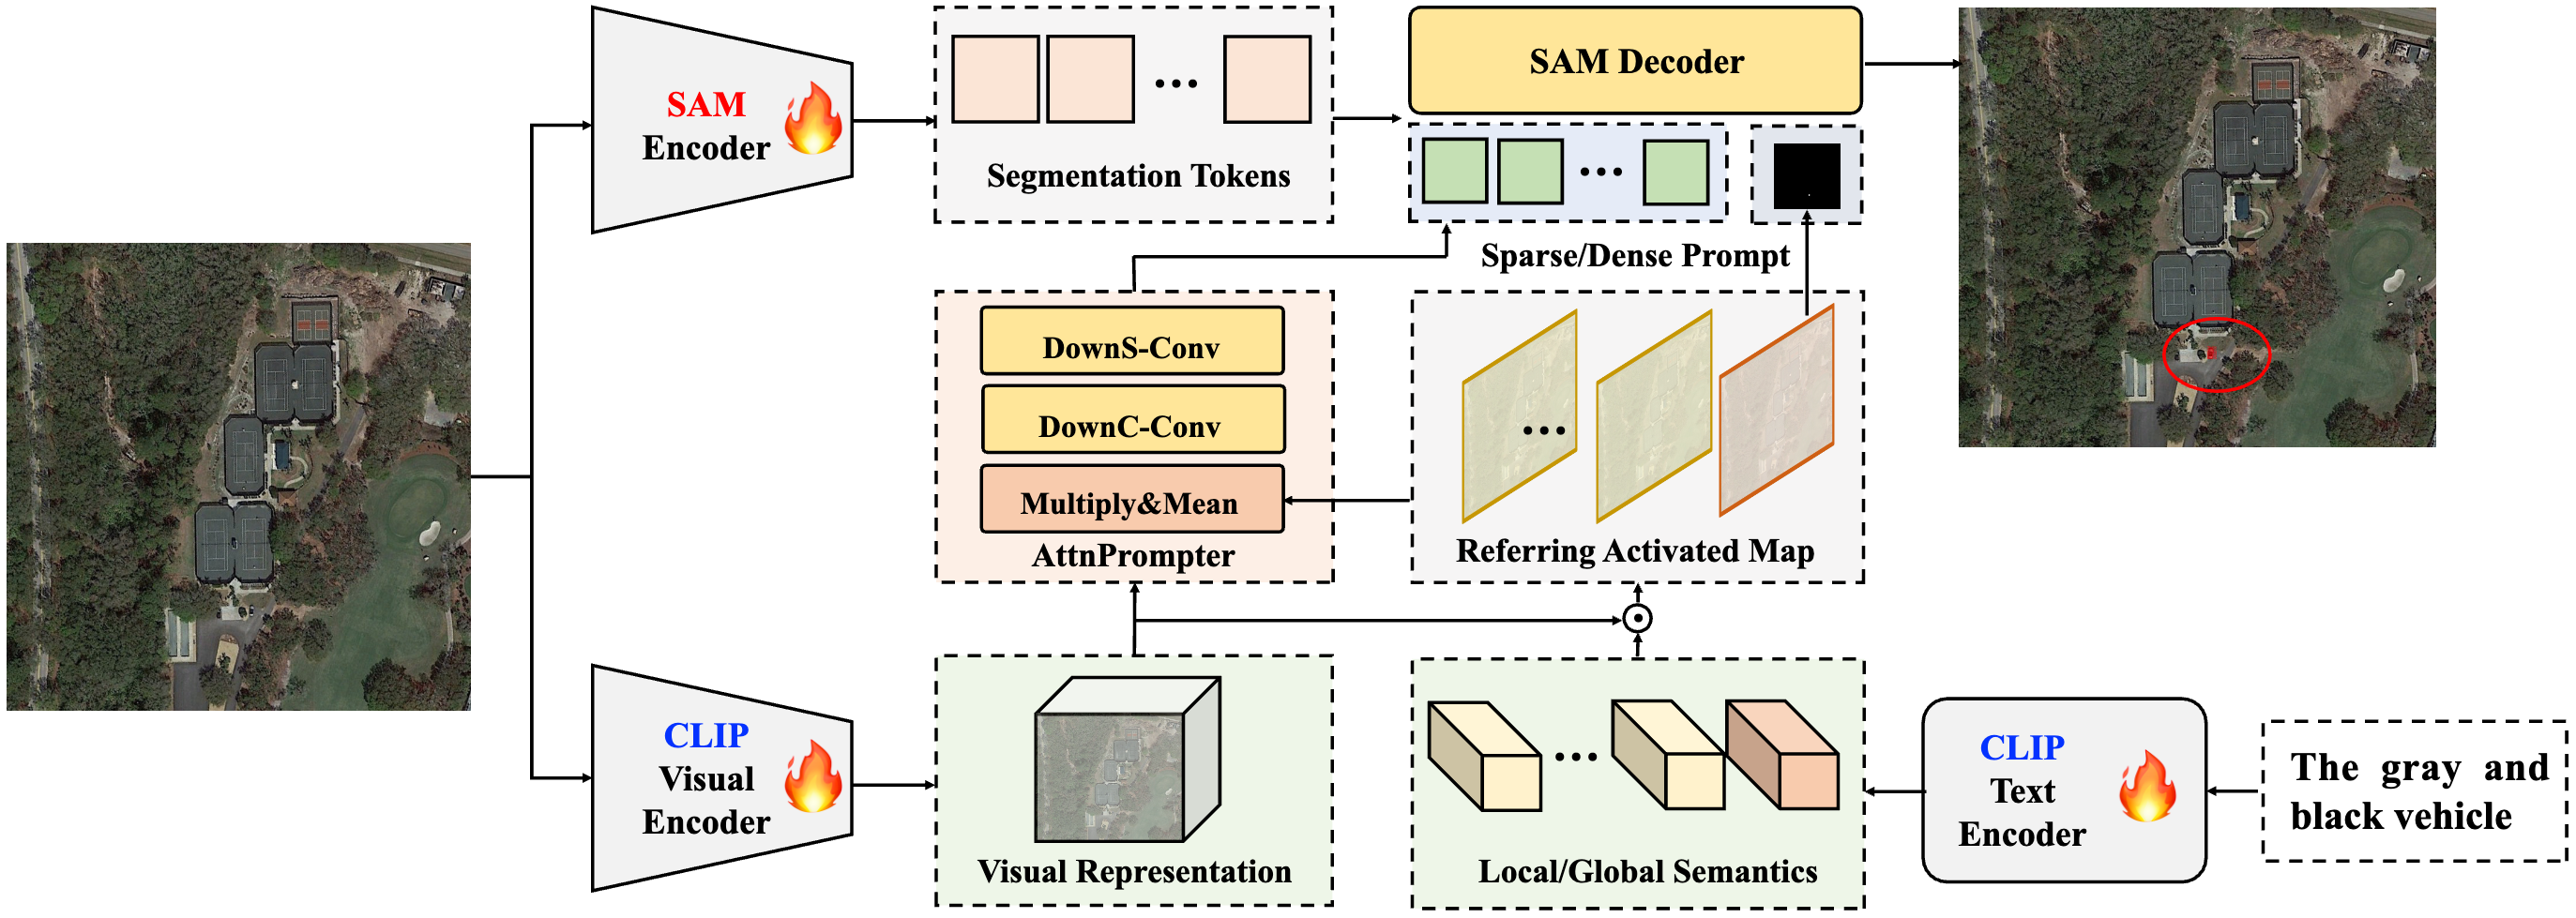
\includegraphics[width=0.9\textwidth]{./Images/RSRefSeg.png}
\caption{RSRefSeg Architecture Overview}
\label{fig:rsrefseg_architecture}
\end{figure}

% #############################################################################
\section{ClipSAM Model Implementation}

We implement a ClipSAM model that leverages SigLIP for multimodal understanding and SAM for precise segmentation mask generation.

\begin{figure}[H]
\centering
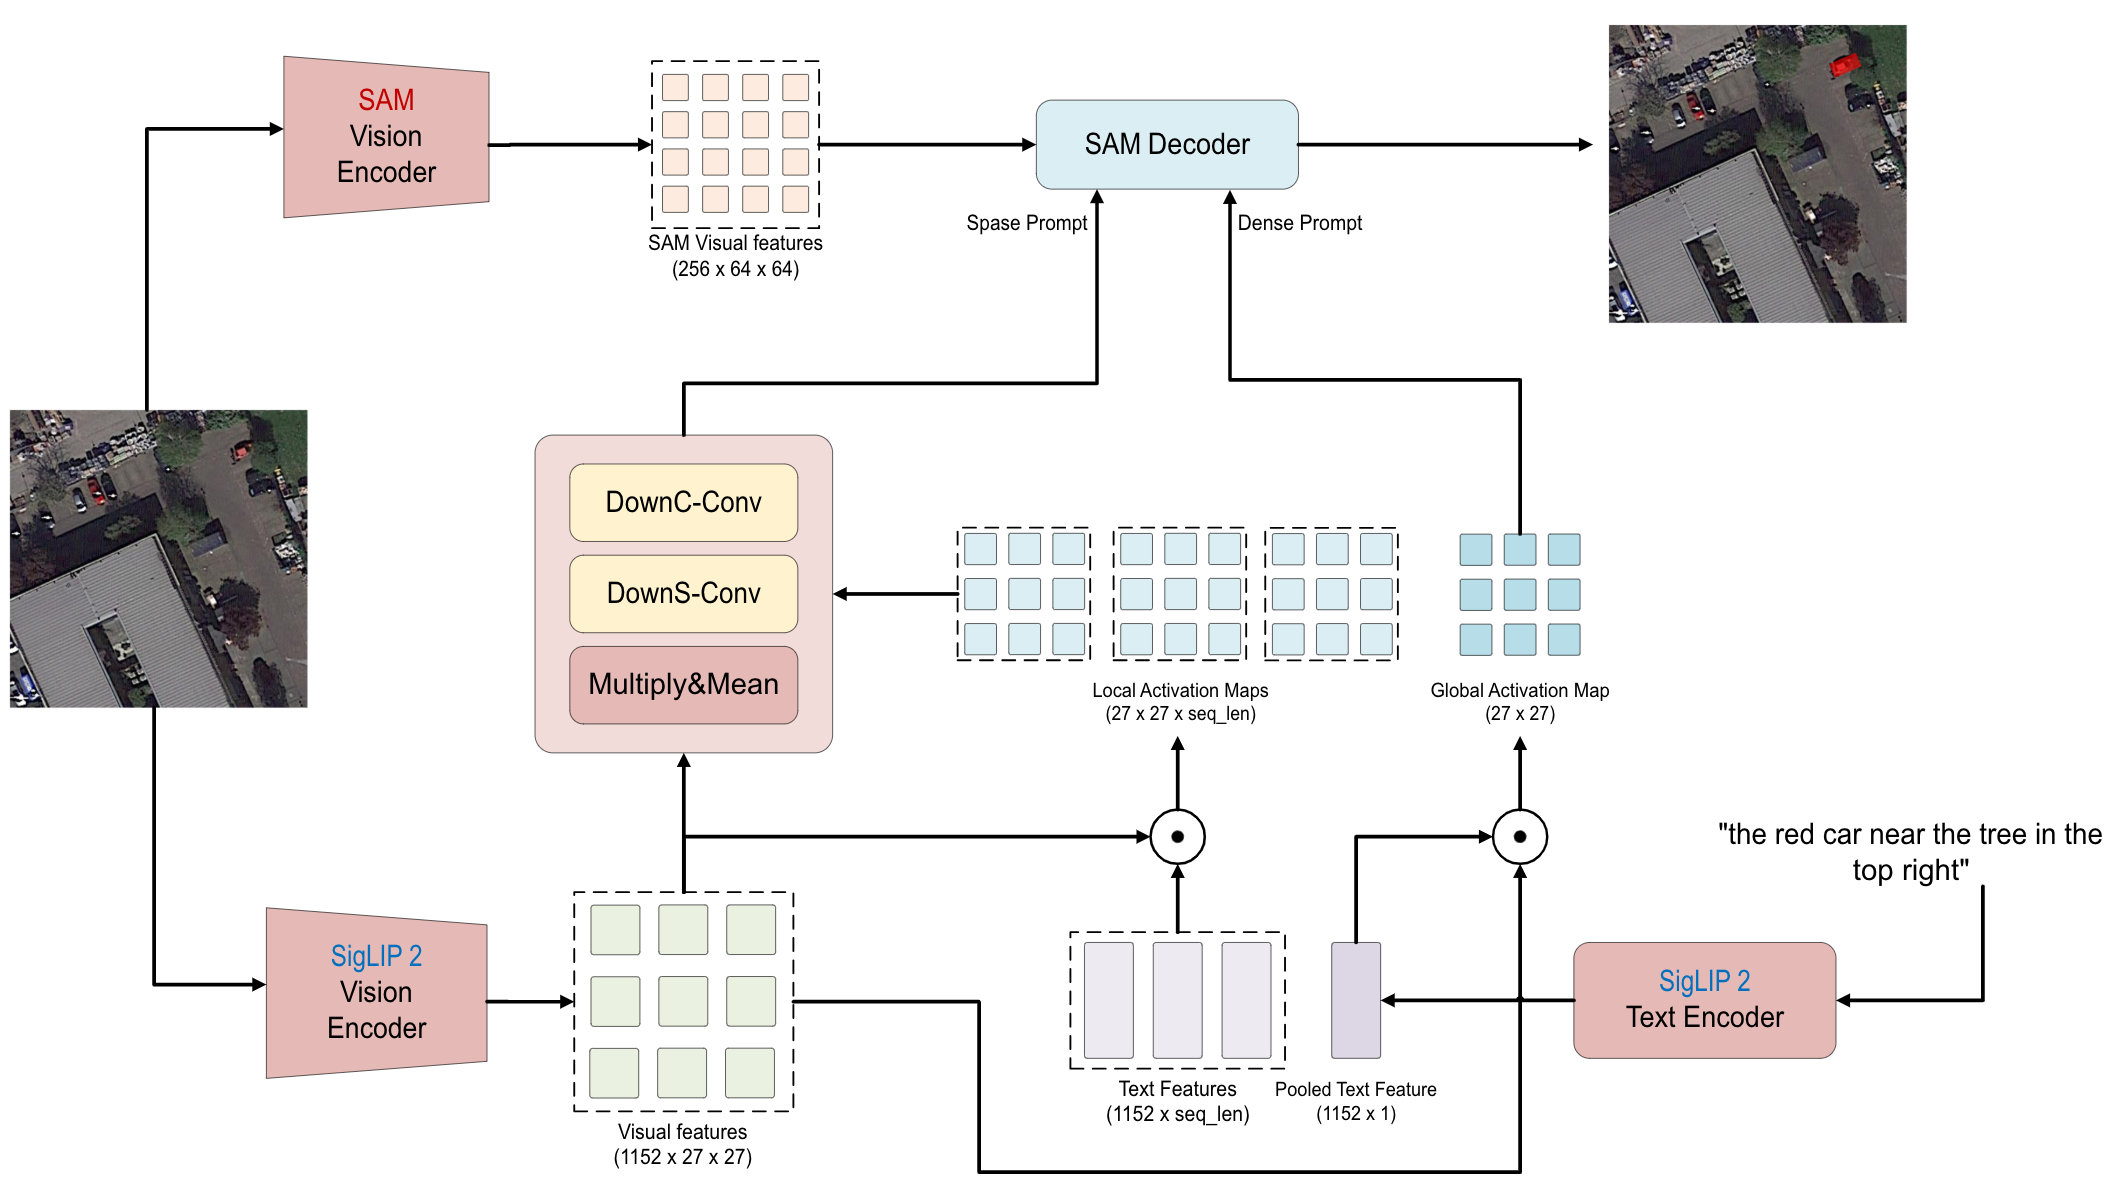
\includegraphics[width=\textwidth]{./Images/clipsam.png}
\caption{ClipSAM architecture overview showing the integration of SigLIP2 vision-language encoder with SAM mask decoder through custom prompter networks for text-guided segmentation. The dual-pathway design processes both local (token-level) and global (sentence-level) text-visual interactions to generate sparse and dense prompts for precise aerial image segmentation.}
\label{fig:clipsam_architecture}
\end{figure}

\subsection{Dataset Statistics}

% Dataset examples figure
\begin{figure}[H]
\centering
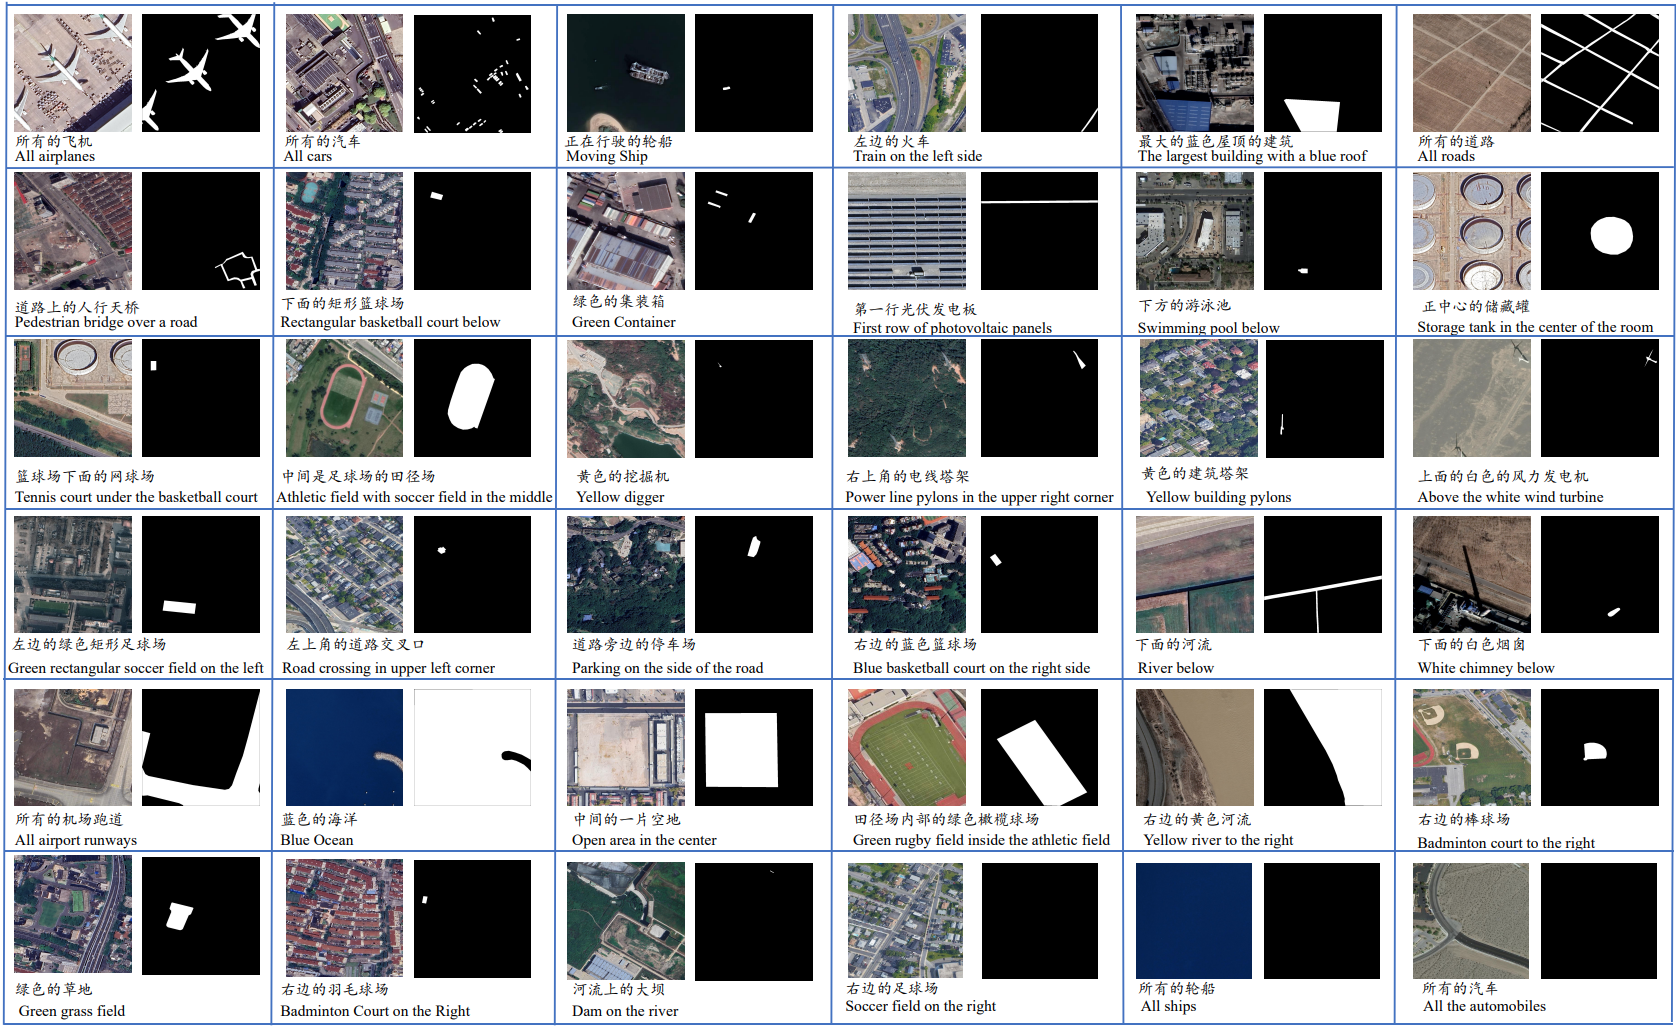
\includegraphics[width=\textwidth]{./Images/dataset.png}
\caption{Representative examples from AERIAL-D dataset showing diverse referring expressions with corresponding aerial images and ground truth masks.}
\label{fig:dataset_examples}
\end{figure}

% Dataset statistics table
\begin{table}[H]
\centering
\caption{Dataset Statistics Summary}
\label{tab:dataset_stats}
\begin{tabular}{@{}lrrr@{}}
\toprule
\textbf{Metric} & \textbf{Train} & \textbf{Val} & \textbf{Total} \\
\midrule
Total Patches & 32,460 & 11,054 & 43,514 \\
Individual Objects with Expressions & 94,179 & 34,536 & 128,715 \\
Individual Expressions & 651,098 & 244,210 & 895,308 \\
Groups with Expressions & 99,986 & 34,216 & 134,202 \\
Group Expressions & 487,214 & 163,472 & 650,686 \\
Total Samples & 1,138,312 & 407,682 & 1,545,994 \\
Avg. Expressions per Individual Object & 6.91 & 7.07 & 6.96 \\
Avg. Expressions per Group & 4.87 & 4.78 & 4.85 \\
\bottomrule
\end{tabular}
\end{table}

\subsection{Category Distribution}

% Category distribution table
\begin{table}[H]
\centering
\caption{Object Category Distribution by Instance Type and Source Dataset}
\label{tab:category_dist}
\resizebox{\textwidth}{!}{%
\begin{tabular}{@{}lrrrrr@{}}
\toprule
\textbf{Category} & \textbf{Individual Instances} & \textbf{Groups} & \textbf{Instance Expressions} & \textbf{Group Expressions} & \textbf{Source Dataset} \\
\midrule
Ship & -- & -- & -- & -- & iSAID \\
Large Vehicle & -- & -- & -- & -- & iSAID \\
Small Vehicle & -- & -- & -- & -- & iSAID \\
Building & -- & -- & -- & -- & iSAID \\
Storage Tank & -- & -- & -- & -- & iSAID \\
Harbor & -- & -- & -- & -- & iSAID \\
Swimming Pool & -- & -- & -- & -- & iSAID \\
Tennis Court & -- & -- & -- & -- & iSAID \\
Soccer Ball Field & -- & -- & -- & -- & iSAID \\
Roundabout & -- & -- & -- & -- & iSAID \\
Basketball Court & -- & -- & -- & -- & iSAID \\
Bridge & -- & -- & -- & -- & iSAID \\
Ground Track Field & -- & -- & -- & -- & iSAID \\
Plane & -- & -- & -- & -- & iSAID \\
Helicopter & -- & -- & -- & -- & iSAID \\
Building & -- & -- & -- & -- & LoveDA \\
Water & -- & -- & -- & -- & LoveDA \\
Barren Land & -- & -- & -- & -- & LoveDA \\
Agricultural Area & -- & -- & -- & -- & LoveDA \\
Forest Area & -- & -- & -- & -- & LoveDA \\
Road & -- & -- & -- & -- & DeepGlobe \\
\bottomrule
\end{tabular}%
}
\end{table}

% #############################################################################
\section{Experimental Configuration} 
This section describes the training configuration and experimental setup for evaluating the RSRefSeg model on the AerialD dataset.

\begin{figure}[h]
\centering
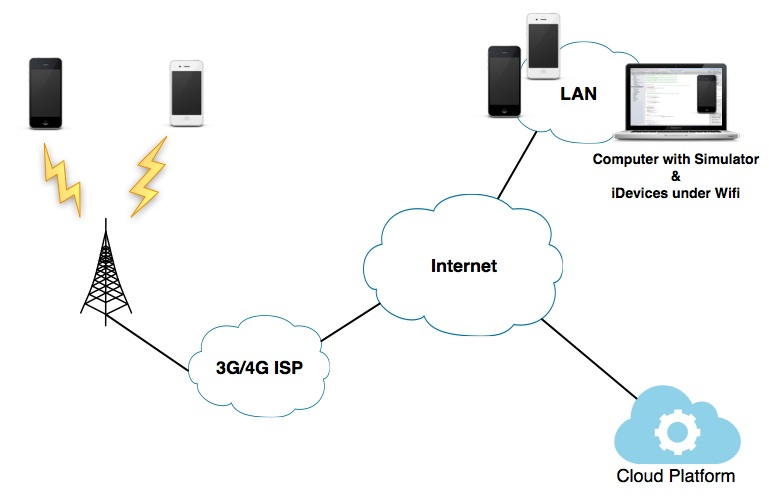
\includegraphics[width=0.8\textwidth]{./Images/test_env}
\caption{Test Environment}
\label{fig:test_env}
\end{figure}

\subsection{Expression Type Analysis}

Table~\ref{tab:expression_type_dist} shows the distribution of different expression types generated across the pipeline, including rule-based expressions and LLM enhancements.

% Expression type distribution table
\begin{table}[H]
\centering
\caption{Expression Type Distribution}
\label{tab:expression_type_dist}
\resizebox{\textwidth}{!}{%
\begin{tabular}{@{}ccccccr@{}}
\toprule
\textbf{Category} & \textbf{Position} & \textbf{Extreme} & \textbf{Size} & \textbf{Color} & \textbf{Relationship} & \textbf{Total Count} \\
\midrule
\multicolumn{7}{l}{\textbf{Rule-Based Individual Instance Expressions}} \\
\midrule
\checkmark & & & & & & -- \\
\checkmark & \checkmark & & & & & -- \\
\checkmark & \checkmark & & & & \checkmark & -- \\
\checkmark & & \checkmark & & & & -- \\
\checkmark & \checkmark & \checkmark & & & & -- \\
\checkmark & \checkmark & \checkmark & & & \checkmark & -- \\
\checkmark & \checkmark & & \checkmark & & & -- \\
\checkmark & \checkmark & & \checkmark & & \checkmark & -- \\
\checkmark & \checkmark & \checkmark & \checkmark & & & -- \\
\checkmark & \checkmark & \checkmark & \checkmark & & \checkmark & -- \\
\checkmark & & & & \checkmark & & -- \\
\checkmark & \checkmark & & & \checkmark & & -- \\
\checkmark & \checkmark & & & \checkmark & \checkmark & -- \\
\checkmark & & \checkmark & & \checkmark & & -- \\
\checkmark & \checkmark & \checkmark & & \checkmark & & -- \\
\checkmark & \checkmark & \checkmark & & \checkmark & \checkmark & -- \\
\checkmark & \checkmark & & \checkmark & \checkmark & & -- \\
\checkmark & \checkmark & & \checkmark & \checkmark & \checkmark & -- \\
\checkmark & \checkmark & \checkmark & \checkmark & \checkmark & & -- \\
\checkmark & \checkmark & \checkmark & \checkmark & \checkmark & \checkmark & -- \\
\midrule
\multicolumn{7}{l}{\textbf{Rule-Based Group Expressions}} \\
\midrule
\checkmark & \checkmark & & & & & -- \\
\checkmark & \checkmark & \checkmark & & & & -- \\
\checkmark & \checkmark & & & & \checkmark & -- \\
\checkmark & \checkmark & & & & \checkmark & -- \\
\checkmark & & & & & & -- \\
\checkmark & & & \checkmark & & & -- \\
\bottomrule
\end{tabular}%
}
\end{table}

\subsection{LLM Enhancement Statistics}

% LLM enhancement stats table
\begin{table}[H]
\centering
\caption{LLM Enhancement Expression Distribution}
\label{tab:llm_enhancement_stats}
\begin{tabular}{@{}lrrr@{}}
\toprule
\textbf{Expression Source} & \textbf{Train} & \textbf{Val} & \textbf{Total} \\
\midrule
Rule-Based Expressions & -- & -- & -- \\
LLM Enhanced (Language Variations) & -- & -- & -- \\
LLM Unique (Visual Details) & -- & -- & -- \\
\midrule
\textbf{Total Expressions} & \textbf{--} & \textbf{--} & \textbf{--} \\
\bottomrule
\end{tabular}
\end{table}

The experimental setup evaluates model performance across different expression types and enhancement levels to understand the impact of each component on segmentation accuracy.

\begin{table}[htb]
\centering
\normalsize
    \caption{Network Link Conditioner Profiles}
    \label{tab:network_profiles}
{\footnotesize
    \begin{tabular}{ | c | c | c | c | }
    \hline 
    \textbf{Network Profile}	& \textbf{Bandwidth} & \textbf{Packets Droped} & \textbf{Delay}\\ \hline \hline
    Wifi  & 40 mbps  &  0\%  &   1 ms \\ \hline
    3G  & 780 kbps  &  0\%  &   100 ms \\ \hline 
    Edge  & 240 kbps  &  0\%  &   400 ms \\ \hline
    \end{tabular}
    }
\end{table}

\subsection{Training Configuration}

% [Training parameters, optimization settings, data splits, augmentation strategies, etc.]

\subsection{Evaluation Methodology}

% [Metrics, validation splits, cross-dataset testing, ablation study design, etc.]
